% !TeX root = ../thuthesis-example.tex
\chapter{随机标准化层}

\section{引言}
本章主要介绍随机标准化层(Stochastic Normalization,StochNorm)的设计思路、具体实现,并且选择少量数据的模型微调场景下进行了相关的实验。

少量数据的模型微调(Small-scale Model Fine-tune)是模型微调中的一个分支,主要的特点在于类别较多、每一类约有10到50条标注数据。
少量数据的模型微调相比小样本学习(Few-shot Learning)来说,每一类的样本数更多,训练得更加充分,得到的模型往往一定程度上能够较好地解决问题;而全量的模型微调中,一般会要求每一类的标注数据足够多,往往多于100条,
这样规模的数据虽然能够使模型获得更好的效果,但是在很多实际场景,如医疗影像数据、工业生产数据的图像识别任务,在训练前期无法获得如此多高质量的标注数据。

如何只利用一定量的高质量标注数据,就能通过模型微调得到效果较为理想的深度学习模型,正是少量数据的模型微调任务所要解决的问题,具有很高的应用价值。同时,在数据量不够充足的情况下,模型微调中存在的很多问题,诸如
灾难性遗忘、负迁移、过拟合、置信度过高等都会愈发严重,因此以少量数据的模型微调场景作为切入点,也具有很高的学术价值。


\section{相关知识}

\subsection{BatchNorm的原理}

BatchNorm在提出之时,作者认为,通过引入这种标准化的机制,能够有效减少深度神经网络的内部协变量偏移(Internal Covariate Shift,ICS)~\citep{ioffe2015BN}。由于深度神经网络涉及到在深度方向多种非线性层的叠加,每一层
的参数更新都会导致输出的数据分布发生变化。由于模型的叠加效应,在网络深处的数据分布变化会变得十分剧烈,因而会使得深度神经网络的训练随着深度的增加变得困难。而在加入BatchNorm之后,每一层输入的数据
会先进行减均值除方差的操作,得到均值为$0$方差为$1$的分布,再通过一组可学习的参数$\beta$和$\gamma$来对数据进行缩放和平移,因此BatchNorm能够动态地调整每一层数据的分布,从而一定程度上避免出现
内部协变量偏移的问题。

随着BatchNorm在深度神经网络中获得巨大的成功,越来越多的人也开始认同BatchNorm通过重参数化(reparameterize)稳定每一层网络的输出来提高网络的性能。然而,学术界一直没有非常完善的实验证明内部协变量偏移
与最终模型效果之间是否有直接的关系,以及BatchNorm是否真的缓解了内部协变量偏移的问题。

\begin{figure}
  \centering
  \subcaptionbox{损失函数Landscape}
    {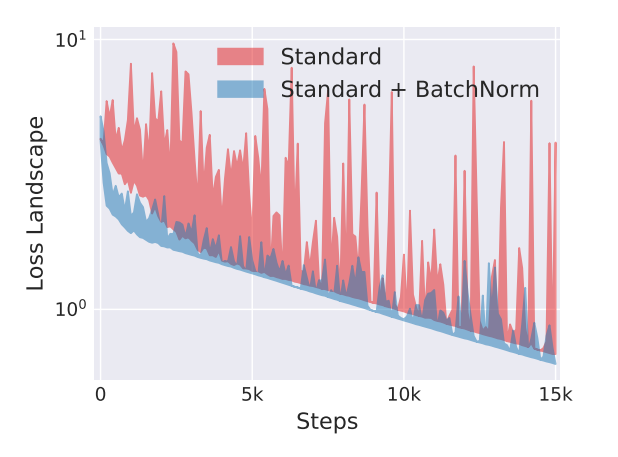
\includegraphics[width=0.46\linewidth]{figures/landscape.png}}
  \subcaptionbox{梯度的可预测性}
    {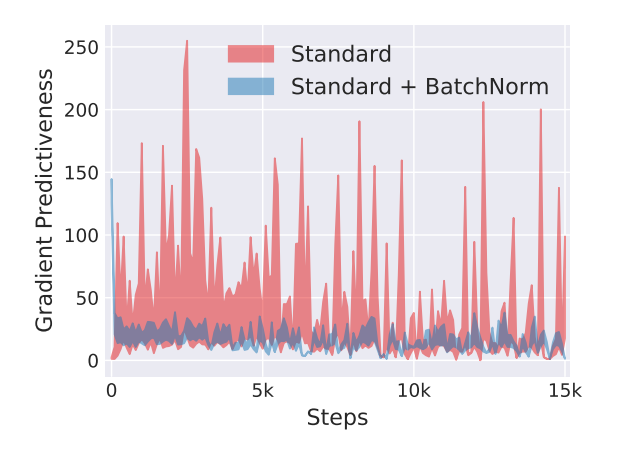
\includegraphics[width=0.47\linewidth]{figures/gradient.png}}
  \caption{BatchNorm对深度神经网络的影响~\citep{santurkar2018does}}
  \label{fig:landsacpe}
\end{figure}

Santurkar~\citep{santurkar2018does}等人的工作通过实验证明,内部协变量偏移与模型最终的效果之间没有必然的联系。作者在原本的BatchNorm的输出后加入了额外的噪声干扰,这些噪声在每一次训练迭代中都
重新生成,因此深度神经网络中每一层在每一个迭代中都有着完全不同的分布。但是添加了噪声之后的模型效果与不添加噪声的对照组相比,并没有明显的变化。同时作者也基于$L_2$距离和余弦距离计算了网络层的
协变量偏移值,发现BatchNorm的引入不会降低,甚至会增加内部协变量偏移值。这些实验证明了,内部协变量偏移与模型的性能没有直接关系,以及BatchNorm并不能显著减少内部协变量偏移。

Shibani Santurkar等人通过理论分析证明,BatchNorm的引入对深度神经网络起到了平滑(Smooth)的作用,使得网络的优化问题对应的空间地貌(landscape)更加平滑,这种影响体现在提升了损失函数的利普希茨性,
获得了更小的利普希茨(Lipschitz)常数:

\begin{definition}[利普希茨常数]
  对于在实数集的子集上定义的映射$f:D \subseteq \mathbb{R} \rightarrow \mathbb{R}$,若存在常数$K$,使得$|f(a)-f(b)| \leq K|a-b| \quad \forall a,b \in D$,则称$f$符合利普希茨条件,
  对于$f$最小的常数$K$成为$f$的利普希茨常数。
\end{definition}

BatchNorm的重参数化使得深度神经网络损失函数对应的梯度的利普希茨常数更小,使得其更加稳定可靠。图~\ref{fig:landsacpe}展示了深度神经网络在加入BatchNorm之后的在损失函数Landscape和梯度可预测性(即
沿着梯度方向梯度的变化值)上的变化。
利普希茨性更好的梯度,使得基于梯度的优化算法能够使用更大的步长进行探索,而不至于发生损失函数突然骤变的现象,例如极其平坦的区域(梯度消失)或尖锐的局部极值(梯度爆炸)。这种性质加速了深度神经网络的训
练,也使其对于学习率等超参数的选择不再那么敏感,从而更容易获得更好的效果。


\subsection{基于正则化的模型微调}
\label{section:regularize}
相比BatchNorm这种从网络结构上进行的正则化约束来说,主流的模型微调方法往往通过在损失函数中加入显式的正则化约束项来进行,以分类任务为例,可以用一个通用的损失函数描述:

\begin{equation}
\label{equal-finetune}
	\mathop {\min} \limits_{ F_{\symup{\Theta}}, G_{\symup{\Theta}}} \sum\limits_{i = 1}^n {\texttt{Loss}(G(F(x_i;F_{\symup{\Theta}});G_{\symup{\Theta}}),y_i)}  + \texttt{Reg} (\cdot)
\end{equation}

其中$x$和$y$表示数据和对应的标签,$F$和$G$分别表示预训练的特征提取器和分类器,$F_{\symup{\Theta}}$和$G_{\symup{\Theta}}$分别表示各自的网络参数,$\texttt{Loss} (\cdot)$表示损失函数,$\texttt{Reg} (\cdot)$表示正则项。
而不同模型微调方法的主要差异则在于对正则项$\texttt{Reg} (\cdot)$的设计,例如如何更大程度利用预训练模型中的知识来设计约束项,从而避免在小的目标域数据集上发生过拟合。

\textbf{$\bm{L_p}$约束 } $L_p$约束中使用模型参数的$L_p$范数作为约束项,是最为经典的一种正则化方法。$L_p$范数的定义如下:

\begin{definition}[$L_p$范数]
  对于$\vec{x}=(x_1, x_2, \cdots ,x_n) \in \mathbb{R}^n$,则$\vec{x}$的$L_p$范数$L_p(\vec{x})={\vert\vert \vec{x} \vert\vert}_p = (\sum_{i=1}^n {\vert x_i \vert}^p)^{\frac{1}{p}} \quad p \geq 1 $
\end{definition}

在深度学习中,一般使用$L_1$和$L_2$范数作为约束项,使用$L_1$范数能够使得深度神经网络获得更好的稀疏性,而模型微调领域中一般使用$L_2$范数:

\begin{equation}
  \texttt{Reg} (F_{\symup{\Theta}}, G_{\symup{\Theta}}) = \frac{1}{\alpha} (\vert\vert F_{\symup{\Theta}} \vert\vert_2^2 + \vert\vert G_{\symup{\Theta}} \vert\vert_2^2) \quad \alpha \in \mathbb{R}
\end{equation}

\textbf{$\bm{L_2}$-SP } $L_2$-SP的目标是缓解模型微调中的灾难性遗忘问题,通过在$L_2$的基础上加入对特征提取器网络参数的约束来实现:

\begin{equation}
  \texttt{Reg} (F_{\symup{\Theta}}, G_{\symup{\Theta}}) = \frac{1}{\alpha} (\vert\vert F_{\symup{\Theta}} \vert\vert_2^2 + \vert\vert G_{\symup{\Theta}} \vert\vert_2^2) + \frac{1}{\beta} \vert\vert F_{\symup{\Theta}} - F_{{\symup{\Theta}}_0} \vert\vert_2^2 \quad \alpha, \beta \in \mathbb{R}
\end{equation}

其中$F_{\symup{\Theta}}$表示特征提取器当前的网络参数,$F_{{\symup{\Theta}}_0}$则表示在预训练模型中特征提取器的网络参数。$L_2$-SP在对网络整体参数做出正则化约束的同时,还迫使特征提取器的参数与预训练模型中不要差异
过大,从而一定程度上避免灾难性遗忘的发生。

\textbf{DELTA } 相较于前面两种作用于网络参数的正则化方法来说,$\rm{DELTA}$则更侧重对深度神经网络获得的特征表征(representation)进行约束,通过引入注意力机制对网络的特征图在特定层进行筛选,对具有更好
迁移性的特征通道赋予更高的注意力权重,第$j$个通道的注意力权重为:


\begin{equation}
\begin{aligned}
  A_j(G,F,F_{{\symup{\Theta}}_0},x_i,y_i) = &\texttt{softmax} (\texttt{Loss}(G(F(x_i; F_{{{\symup{\Theta}}_0}\backslash j});G_{{{\symup{\Theta}}_0}\backslash j}), y_i) \\ 
  &-\texttt{Loss}(G(F(x_i; F_{{\symup{\Theta}}_0});G_{{\symup{\Theta}}_0}), y_i)) \\
\end{aligned}
\end{equation}

其中$F_{{{\symup{\Theta}}_0}\backslash j}$和$G_{{{\symup{\Theta}}_0}\backslash j}$表示去除第$j$个通道网络参数的特征提取器和分类器,最终的正则化约束项为:

\begin{equation}
\begin{aligned}
  \texttt{Reg} (F_{\symup{\Theta}}, G_{\symup{\Theta}}) &= \frac{1}{\alpha} (\vert\vert F_{\symup{\Theta}} \vert\vert_2^2 + \vert\vert G_{\symup{\Theta}} \vert\vert_2^2) + \frac{1}{\beta} \sum_{i=1}^{m}\sum_{j=1}^{N} { 
    A_j(G,F,F_{{\symup{\Theta}}_0},x_i,y_i) \texttt{Reg}(f_j)}  \\
    \texttt{Reg}(f_j) &= \vert\vert f_j(F,F_{{\symup{\Theta}}}, x_i) - f_j(F,F_{{\symup{\Theta}}_0},x_i) \vert\vert_2^2 \quad \alpha, \beta \in \mathbb{R} \\
\end{aligned}
\end{equation}

其中$f_j$表示网络特定层输出特征图的第$j$个通道。

\textbf{BSS } 尽管模型微调场景下大多数的正则化方法都是针对灾难性遗忘问题而提出,也有一部分工作面向负迁移(Negative Transfer)问题。BSS(Batch Spectral Shrinkage)~\citep{chen2019catastrophic}
中参考主角(Principal Angles)分析提出了一致角(Corresponding Angles)的概念,通过度量两个矩阵的特征向量之间的余弦距离,来刻画特征图矩阵不同特征向量的迁移性,即不同领域间一致角越小的特征向量具有越好
的迁移性。BSS首先对特征提取器输出的特征进行奇异值分解(Singular Value Decomposition,SVD):
\begin{equation}
  F(\symbf{x}) = \symbf{\symup{U\Sigma V^\top}}
  % \symbf{\symup{\Sigma}} &= (\sigma_1, \sigma_2, \cdots, \sigma_n) \\
\end{equation}

之后基于分解得到的奇异值对网络的训练进行正则化约束:

\begin{equation}
  \texttt{Reg} (\cdot) = \alpha \sum_{i=1}^k \sigma_{-i}^2 \quad \alpha \in \mathbb{R} \\
\end{equation}

其中$k$表示要进行约束的奇异值的数量,而$\sigma_{-i}$表示第$i$小的奇异值。

总的来说,正则项$\texttt{Reg} (\cdot)$的引入更偏向于一种强制性的约束,迫使深度神经网络的训练满足某种条件,从而一定程度上避免在模型微调中遇到的灾难性遗忘或者负迁移的问题。
但是这些约束条件往往需要进行巧妙的设计,同时使用一定的超参数与原始的损失函数进行权衡,否则会对网络的训练产生过大的影响,甚至带来负面的影响。

\section{随机标准化层}

本文提出的随机标准化层(Stochastic Normalization)是以深度神经网络中使用非常广泛的BatchNorm为基础,通过引入双分支结构和随机前馈机制设计的新的标准化层结构。

\subsection{BatchNorm在模型微调中的不足}

尽管BatchNorm被广泛应用在深度神经网络中,它依然存在着很多的缺陷。在训练阶段,BatchNorm的输出依赖于这一批数据的均值和方差,而真正用于估计数据分布的期望和方差的$\tilde{\mu}$和$\tilde{\sigma}^2$则只在推理阶段被使用。这意味着
包含BatchNorm的深度神经网络的训练容易过分依赖批数据的期望和方差,从而影响网络泛化性。尤其在训练样本总数较少或者每一批数据内部差异较小的情况下,这一批数据的均值和方差会存在较大的误差。


BatchNorm目前被广泛应用于各种深度神经网络结构的训练当中,在数据量以及Batch Size都足够大的情况下,往往能取得非常好的效果。这是由于足够大的Batch Size能够使BatchNorm中用于训练阶段标准化的统计量
$\mu$和$\sigma^{2}$更加准确可靠,而足够大的数据量能够使用于预测阶段标准化的统计量$\tilde{\mu}$和$\tilde{\sigma}^{2}$更好地估计整体数据分布的期望和方差,两个条件的满足保证了BatchNorm的效果。
在物体检测领域中,由于GPU计算能力以及显存的限制,Batch Size往往只有个位数,此时$\mu$和$\sigma^{2}$的估计就容易产生较大误差,因此一般使用改进的Batch Norm或者换用其他标准化层。

而在图像分类任务中,常规的GPU显存足以容纳足够大的Batch Size用于训练,因此前者的估计依然得以保证,但是在模型微调场景下往往只有很少量的有标注数据,相比起预训练阶段要少得多,导致$\tilde{\mu}$和$\tilde{\sigma}^{2}$
的估计容易出现偏差,考虑到BatchNorm在推理阶段使用这两个估计值来估计数据分布的期望和方差,BatchNorm很容易在一些模型微调场景下无法获得很好的效果。

除此之外,相较于常规的从头训练而言,预训练模型在模型微调场景中的作用不可忽视。但是在传统的模型微调场景下,深度神经网络会使用预训练模型的网络参数进行初始化,但是一般只包括特征提取器中的可学习参数,
而BatchNorm中的$\tilde{\mu}$和$\tilde{\sigma}^{2}$则是通过滑动平均的方式进行更新的得到的,属于不可学习的统计量,因此在模型微调时,预训练模型在预训练数据上更新得到的$\tilde{\mu}$和$\tilde{\sigma}^{2}$
会被直接丢弃。但是对于基本收敛的预训练模型而言,每一层网络层的输入输出与BatchNorm的标准化过程相互耦合,如果直接丢弃这些滑动平均的统计值,便无法充分利用预训练模型中的知识,往往会在训练初期导致
可学习参数与BatchNorm之间的不匹配(mismatch)。

% 在节~\ref{section:problem}中提到的

% BatchNorm目前被广泛应用于各种深度神经网络结构的训练当中,在数据量$n$以及Batch Size$m$都足够大的情况下,往往能取得非常好的效果。这是由于足够大的$m$能够使BatchNorm中的
% $(\mu, \sigma^{2})$更加准确可靠,而足够大的$n$能够使$(\tilde{\mu}, \tilde{\sigma}^{2})$更好的估计数据分布$P$的期望和方差,
% 但是Batch Size $m$往往依赖于图形处理器(Graph Processing Unit,GPU)的计算能力以及显存,在很多实际场景中并不会很大,例如在物体检测(Object Detection)中,单张图形处理器上
% 的Batch Size $m$一般很难超过$10$。而在图像分类(Image Classification)任务中,$m$往往是几十甚至几百,因此BatchNorm可以很好地对$(\mu, \sigma^{2})$进行计算。但是在模型微调
% 场景下,数据量$n$相比起预训练阶段来说要小得多,如果数据量不够充足,往往BatchNorm无法获得很好的效果。

\subsection{双分支结构}

为了解决上一节提到的BatchNorm在模型微调场景下存在的问题,我们将标准化的过程分为两个分支,一个分支仍然使用BatchNorm的计算方式,另一个分支则使用网络当前估计得到的$\tilde{\mu}$和方差$\tilde{\sigma}^2$来进行标准化:
\begin{equation}
  \label{equal-sn_mean&var}
  \begin{aligned}
    \widehat{x}_{i,0}=\frac{x_{i}-\tilde{\mu}}{\sqrt{\tilde{\sigma}^{2}+\epsilon}},\quad
    \widehat{x}_{i,1}=\frac{x_{i}-\mu}{\sqrt{\sigma^{2}+\epsilon}}.
  \end{aligned}
\end{equation}

\begin{figure}
  \centering
  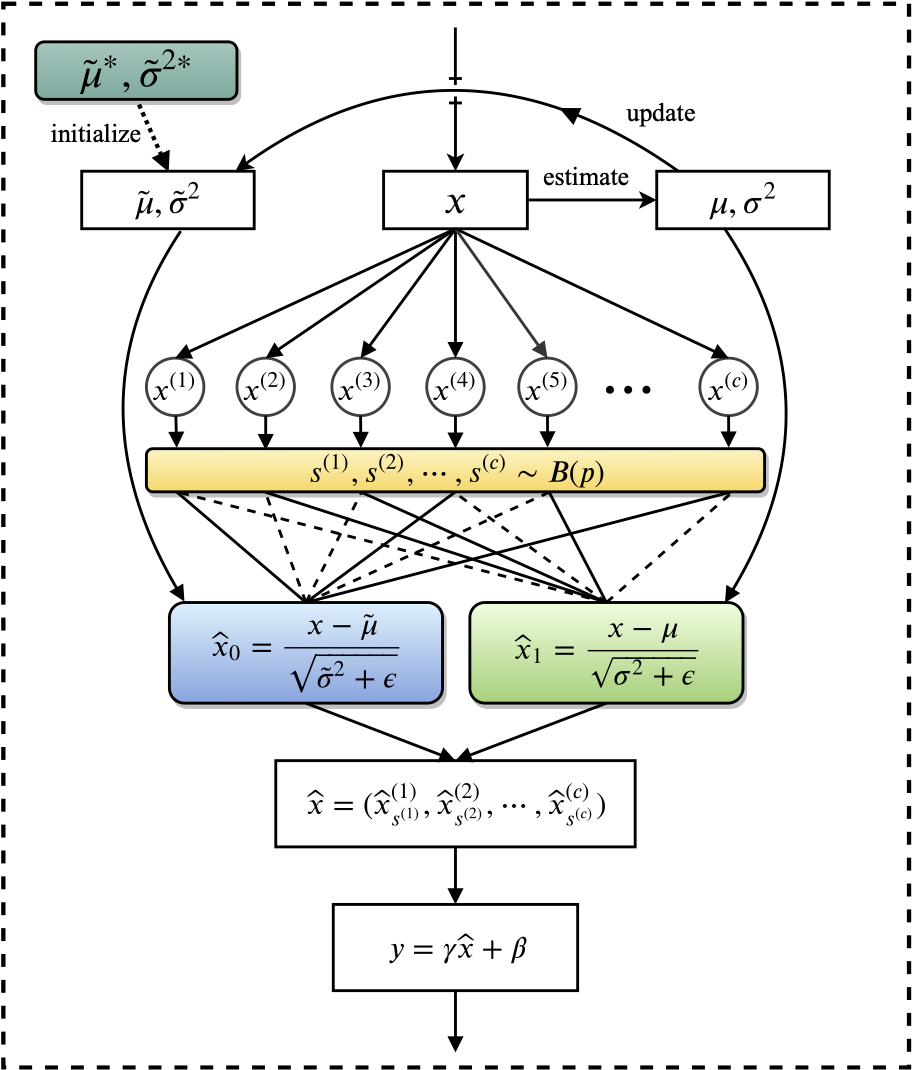
\includegraphics[width=0.7\linewidth]{figures/arch.png}
  \caption{StochNorm的整体结构}
  \label{fig:arch}
\end{figure}

下一步是基于某个概率$p$对两个分支对特征图进行标准化的结果进行选择。令$s$表示最终选择的分支,则$x_{i,s}$表示传入下一步的标准化特征图。本文采用伯努利分布(Bernoulli Distribution)

\begin{equation}
  P(s)=\left\{
  \begin{matrix}
    p, & s=1\\ 
    1-p,  & s=0
  \end{matrix}
  \right.
\end{equation}

对两个分支的标准化结果进行随机选择,这一选择的过程可以表示为:

\begin{equation}
  \widehat{x}_{i}=(1-s)\widehat{x}_{i,0}+s\widehat{x}_{i,1}
\end{equation}

之后依旧按照BatchNorm的操作,使用参数$\beta$和$\gamma$对$\widehat{x}_{i}$进行缩放的平移。

通过伯努利分布的概率$p$,我们可以根据实际场景来平衡个分支的输出。当$p=1$时,StochNorm退化为BatchNorm,但是当训练数据较少时,传统的基于BatchNorm的训练很容易出现过拟合;而$p=0$时,会完全依赖滑动平均估计的统计值进行标准化,
即使在输入数据统计值有明显差异的情况下,依旧会强迫深度神经网络根据滑动平均估计得到的均值和方差进行标准化。但是通过引入随机选择的机制,StochNorm能够让网络在训练过程中,既不会完全忽视输入数据的统计特征,也不会过分拟合,这种标准化层
结构以一种类似Dropout~citep{}的方式对深度神经网络的训练实现了正则化约束,从而一定程度上避免了过拟合的发生,提升了模型的效果。

StochNorm的整体结构如图~\ref{fig:arch}所示,其中$c$表示输入的特征图$x$的通道数,$j$表示通道的小标,$\tilde{\mu}^*, \tilde{\sigma}^{2^*}$表示预训练模型中的滑动平均估计的统计值。在推理阶段,黄色和绿色的模块将不被使用。StochNorm的具体的计算过程如算法~\ref{alg:main}所示。

\subsection{更充分地利用预训练模型参数}

% 统计量和模型网络的耦合

在节~\ref{section:bn}中提到,BatchNorm中的$\tilde{\mu}, \tilde{\sigma}^2$对实际的网络训练过程没有影响。因此尽管在预训练模型中也保存了过去更新得到的$\tilde{\mu}^*, \tilde{\sigma}^{2^*}$,
由于BatchNorm的机制,这些参数对模型微调阶段没有帮助。同时,由于BatchNorm中使用滑动平均的方式对两个估计值进行更新,初始值的影响也随着训练的进行不断减小。尽管并非是可学习的网络参数,
$\tilde{\mu}, \tilde{\sigma}^2$也是通过预训练数据,以及预训练数据上学习得到的可学习网络参数计算得到的,理所当然地包含着许多预训练数据中有价值的知识,但是现有的方法中直接忽略了这些知识。

在StochNorm中,由于双分支结构的巧妙设计,存在着一支使用$\tilde{\mu}, \tilde{\sigma}^2$进行标准化的分支,可以自然而然地使用$\tilde{\mu}^*, \tilde{\sigma}^{2^*}$作为其初始值,如图~\ref{fig:arch}中
左上角所示。通过这种方式,StochNorm使得预训练模型中的滑动平均估计的统计值也能够参与训练,对模型微调的最终效果起到帮助。这种初始化的策略也对网络的训练起到了隐式的正则化约束。

\begin{algorithm}[htbp]
  \caption{随机标准化层 (StochNorm)}
  \label{alg:main}
  \begin{algorithmic}
      \STATE \hspace{-11pt} {\bfseries 输入}: 一批数据内每个通道的特征图 $x=\{x_{i}\}_{i=1}^{m}$;\\
      (BatchNorm) 滑动平均更新速率 $\alpha \in (0,1)$ 和可学习参数 $\beta, \gamma$;\\
      (StochNorm) 滑动平均估计的统计值 $\tilde{\mu}, \tilde{\sigma}^2$ (初始值为 $\tilde{\mu}^*, \tilde{\sigma}^{2^*}$) 和分支选取概率 $p \in (0,1)$。 \\
      \STATE \hspace{-11pt} {\bfseries 输出}: $y={\textrm{StochNorm}}(x)$.。
  
      \STATE \hspace{-11pt} \textbf{训练阶段:}
      \STATE $\displaystyle \mu \leftarrow \frac{1}{m}\sum_{i=1}^{m}x_{i}, \quad \sigma^2 \leftarrow \frac{1}{m}\sum_{i=1}^{m}(x_i-\mu)^2$ \hfill $//$ \textit{计算均值和方差}
      \setstretch{1.4}
  
      \STATE $\displaystyle \widehat{x}_{i,0} \leftarrow
      \frac{x_{i}-\tilde{\mu}}{\sqrt{\tilde{\sigma}^2+ \epsilon}}$
      \hfill $//$ \textit{使用滑动平均估计的统计值进行标准化}
      
      \STATE $\displaystyle \widehat{x}_{i,1} \leftarrow 
      \frac{x_{i}-\mu}{\sqrt{\sigma^2+\epsilon}}$
      \hfill $//$ \textit{使用批数据统计值进行标准化}

      \STATE $\widehat{x}_{i}=(1-s)\widehat{x}_{i,0}+s\widehat{x}_{i,1}, \quad s \sim B(p)$
      \hfill $//$ \textit{对每个通道进行随机的分支选取}
      
      \STATE $y_{i} \leftarrow \gamma \widehat{x}_{i} +\beta$
      \hfill $//$ \textit{伸缩与平移}
      \STATE $\tilde{\mu} \leftarrow \tilde{\mu} + \alpha (\mu-\tilde{\mu}), \quad \tilde{\sigma}^2 \leftarrow \tilde{\sigma}^2 + \alpha (\sigma^2-\tilde{\sigma}^2)$ 
      \hfill $//$ \textit{滑动平均更新估计值}
      
      \STATE \hspace{-11pt} {\bfseries 推理阶段:}
      \STATE $\displaystyle y_{i} \leftarrow \gamma \frac{x_{i}-\tilde{\mu}}{\sqrt{\tilde{\sigma}^2 + \epsilon}} + \beta$ \hfill $//$ \textit{使用滑动平均估计值进行标准化}
  \end{algorithmic}
\end{algorithm}

总的来说,StochNorm从两个方面使得模型微调具有更好的鲁棒性和泛化性:双分支的结构设计加上随机选取分支进行标准化的机制,实现了两种标准化方式的结合,对模型微调阶段起到了正则化的约束效果;
将预训练模型中的非可学习参数$\tilde{\mu}^*, \tilde{\sigma}^{2^*}$利用了起来,更大程度上迁移了预训练模型中的知识。
同样的,由于在训练阶段引入了通过$\tilde{\mu}^*, \tilde{\sigma}^{2^*}$进行标准化的分支,StochNorm进一步缓解了在节~\ref{section:problem}中提到的训练和预测阶段标准化方式不一致导致的问题。 


% \begin{itemize}
%   \item 双分支的结构设计加上随机选取分支进行标准化的机制,实现了两种标准化方式的结合,对模型微调阶段起到了正则化的约束效果;
%   \item 将预训练模型中的非可学习参数$\tilde{\mu}^*, \tilde{\sigma}^{2^*}$利用了起来,更大程度上迁移了预训练模型中的知识。
% \end{itemize}



\subsection{使用随机标准化层进行模型微调}

本节介绍StochNorm的主要应用方式和场景,包括与其他主流模型微调方法或者深度神经网络结构相结合,进一步提升模型微调的效果。

\textbf{与主流模型微调方法相结合 } 在节~\ref{section:regularize}中提到的,主流的基于正则项的模型微调方法,一般会在模型层面外,对训练时的损失函数进行修改,而且更偏向于一种显式的目的性较强的约束。
StochNorm则通过结构上的巧妙设计,隐式地提升了深度神经网络的迁移能力,同时起到正则化约束的效果。这两种方式是相互正交、相互补充的,通过将特征提取器$F$中的BatchNorm替换为StochNorm,
便可以同时获得两种正则化效果,进一步提升模型的最终效果,在节~\ref{section:ablation}中有更详细的实验验证。

\textbf{与主流深度神经网络结构相结合 } 作为一种通用并且轻量的标准化层结构,StochNorm可以被非常轻松地加入各种主流的使用了BatchNorm的深度神经网络结构中,只需要直接将BatchNorm替换为StochNorm即可。
如图~\ref{fig:integratio}所示,StochNorm可以应用在多种主流深度神经网络结构中,如VGG-16~\citep{simonyan2015very},ResNet~\citep{he2016deep}以及Inception Net~\citep{szegedy2016rethinking},
而不需要修改其他组件。

\begin{figure}
  \centering
  \subcaptionbox{VGG Block}
    {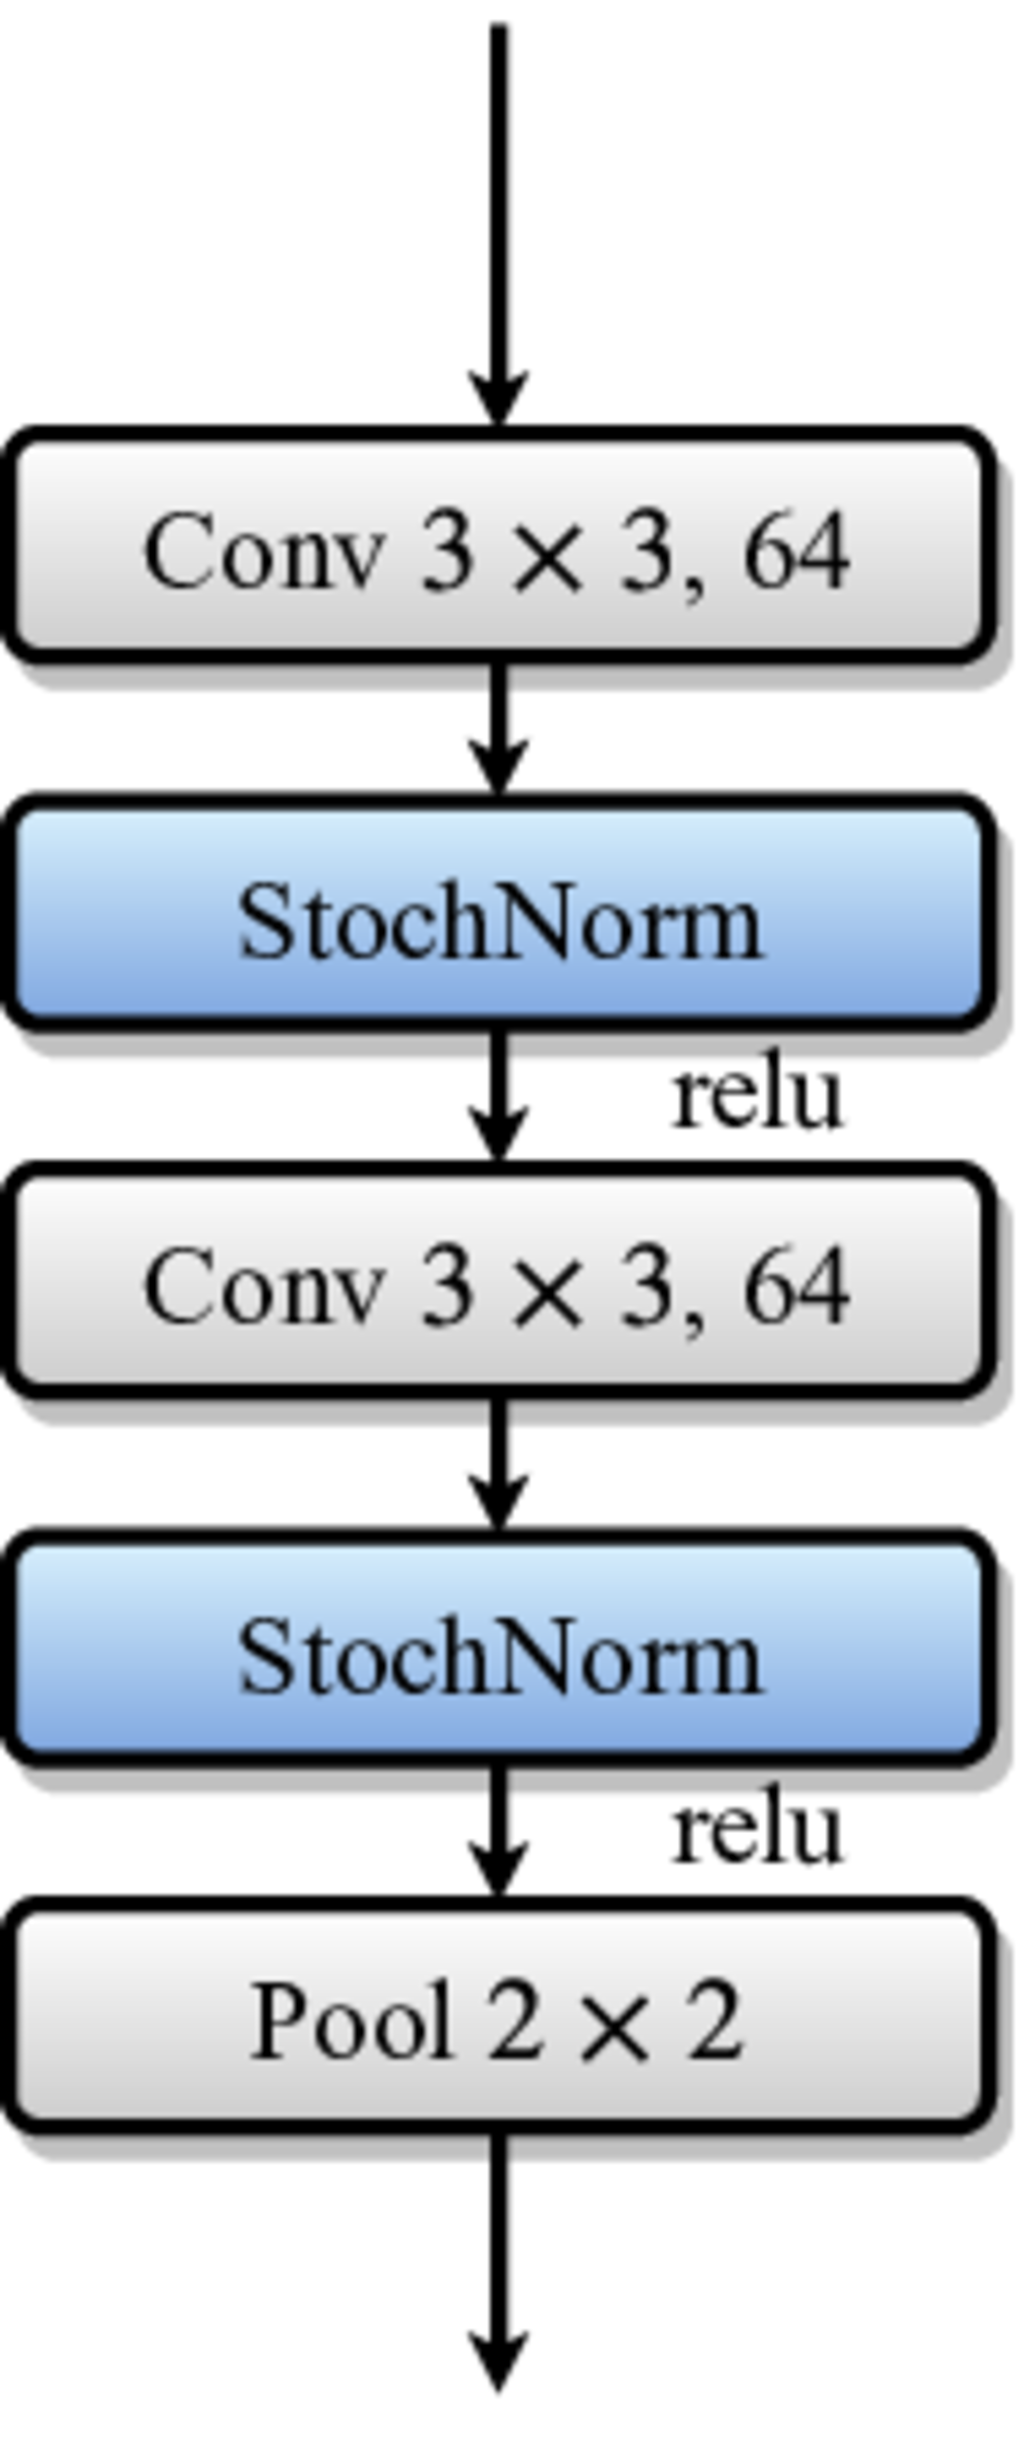
\includegraphics[width=0.16\linewidth]{figures/vgg-block.png}}
  \hspace{15pt}
  \subcaptionbox{Residual Block}
    {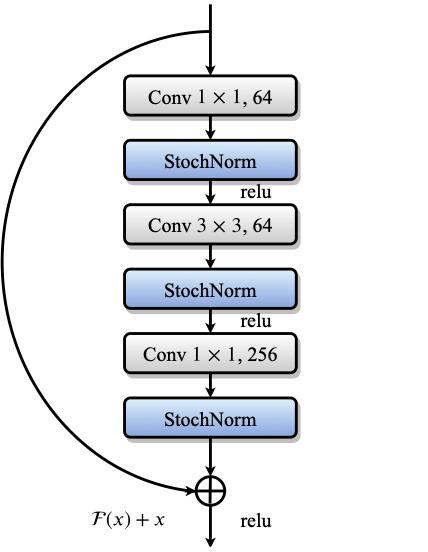
\includegraphics[width=0.29\linewidth]{figures/resnet-block.png}}
  \subcaptionbox{Inception Block}
    {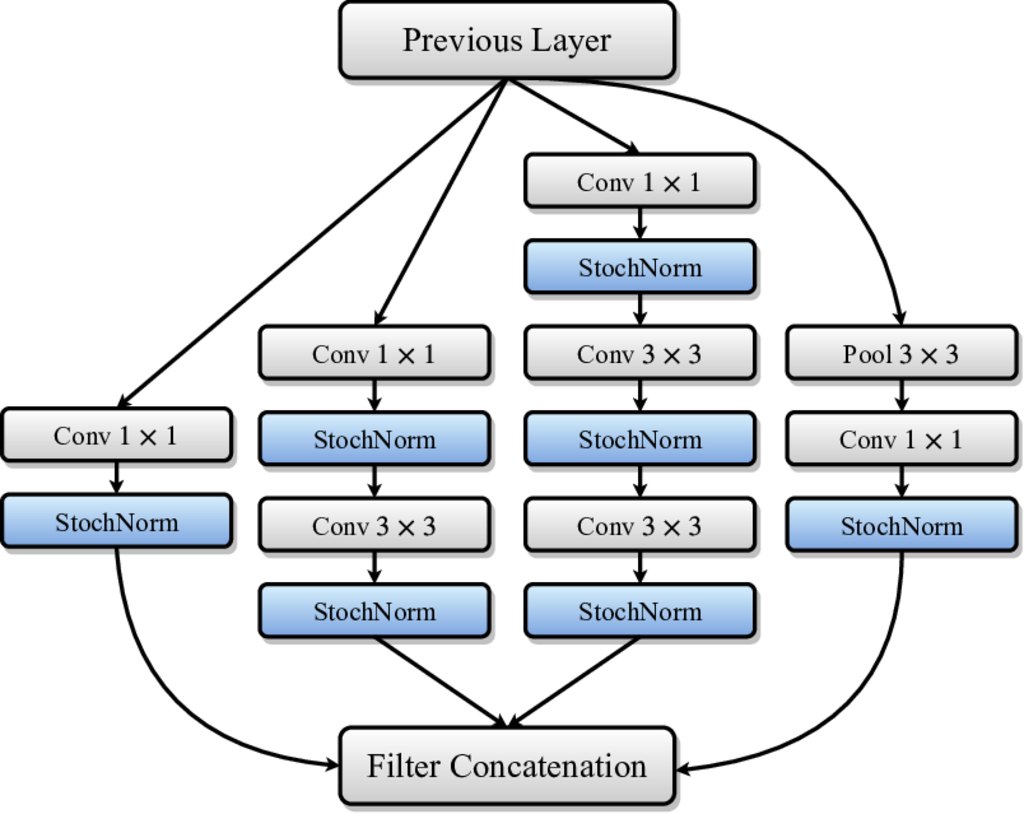
\includegraphics[width=0.44\linewidth]{figures/inception-block.png}}
  \caption{在主流深度神经网络结构中使用StochNorm}
  \label{fig:integratio}
\end{figure}


\section{实验}

\subsection{实验设计}
\label{section:settings}

\textbf{深度学习框架 } 随着深度学习的不断发展,研究人员们也相应开发了各式各样的深度学习框架,逐渐成为了深度学习不可或缺的一部分。目前学术界主流的深度学习框架为TensorFlow[引]和PyTorch\citep{benoit_pytorch:_2019}。
PyTorch使用了动态的计算图,使用方法很接近原生的Python语言,具有效率高、可读性强等优点,逐渐成为学术界使用最为广泛的深度学习框架。因此本文使用PyTorch来进行相关的实验。

\textbf{实验环境 } 本文的所有实验均使用装有8块GPU的深度学习服务器来进行,服务器的详细配置如表~\ref{table:server-setting}所示。

\begin{table*}[h]
	\begin{center}
	\caption{服务器配置信息}
	\label{table:server-setting}
    \begin{tabular}{ll}
        \toprule
        项目 & 配置信息 \\
        \midrule
        操作系统 & Ubuntu 18.04.3 LTS \\
        中央处理器 & Intel(R) Xeon(R) Gold 6130 CPU @ 2.10GHz \\
        中央处理器核心数 & 64 \\
        内存 & 32GB \\
        图形处理器 & NVIDIA TITAN X \\
        显存 & 12GB \\
        Python版本 & 3.8.10 \\
        PyTorch版本 & 1.9.0 \\
        CUDA版本 & 11.2 \\
        \bottomrule
    \end{tabular}
	\end{center}
\end{table*}

\textbf{数据集 } 本文在三个细粒度分类数据集上进行了模型微调相关的实验:\textbf{CUB-200-2011 }~\citep{WelinderEtal2010}是一个鸟类图片的细粒度分类数据集,包含一共$200$种鸟类,共$11788$张图片,是CUB-200数据集
的扩展版本;\textbf{Standford Cars }~\citep{KrauseStarkDengFei-Fei_3DRR2013}是一个车辆图片的细粒度分类数据集,包含一共$196$种车辆,共$16185$张图片;\textbf{FGVC Aircraft }~\citep{maji2013fine}是一个航空飞行器的细粒度分类数据集,包含$102$种飞行器,共$10200$张
图片。三个数据集的部分图片如图~\ref{fig:datasets}所示。可以看出,三个数据集都属于同一大类下不同细分类别的图像分类问题,具有图片规模较小、类间差异较小等特点,很适合作为验证模型微调方法的评测数据集。

\begin{figure}
  \centering
  \subcaptionbox{CUB-200-2011}{
    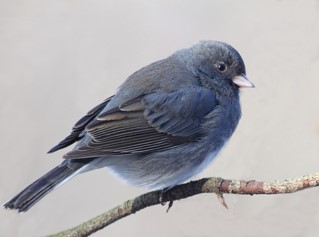
\includegraphics[width=0.271\linewidth]{figures/cub/1.jpg}
    
\includegraphics[width=0.3\linewidth]{figures/cub/4.jpg}
    
\includegraphics[width=0.305\linewidth]{figures/cub/3.jpg}
  }
  \subcaptionbox{Standford Cars}{
    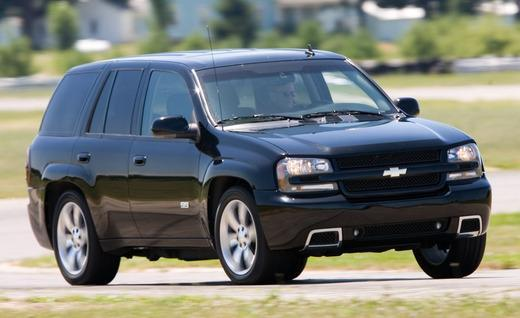
\includegraphics[width=0.3\linewidth]{figures/car/1.jpg}
    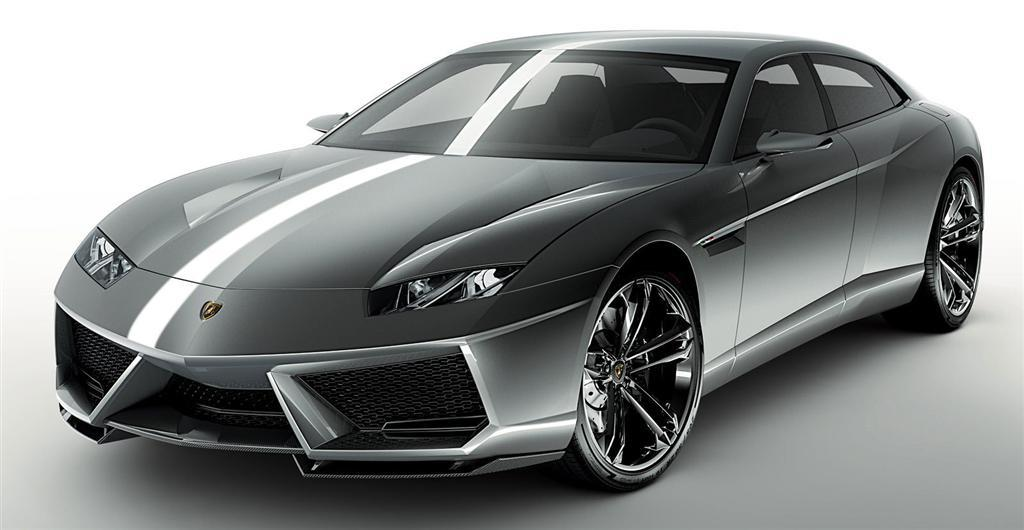
\includegraphics[width=0.3\linewidth]{figures/car/2.jpg}
    
\includegraphics[width=0.3\linewidth]{figures/car/3.jpg}
  }
  \subcaptionbox{FGVC Aircraft}{
    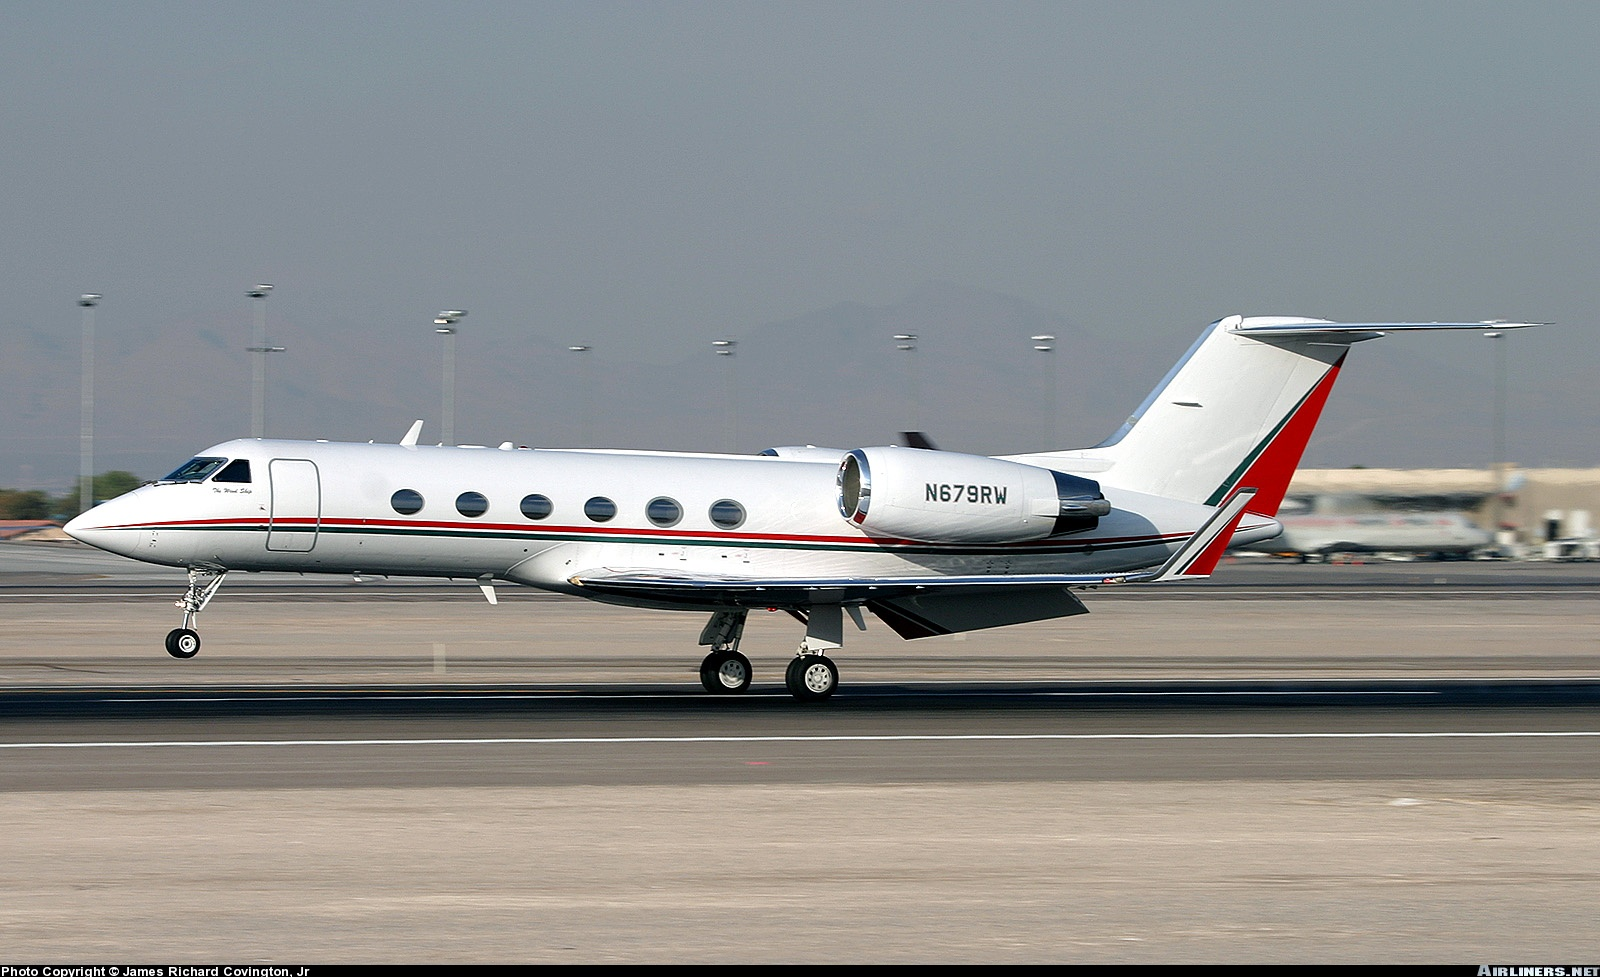
\includegraphics[width=0.335\linewidth]{figures/air/1.jpg}
    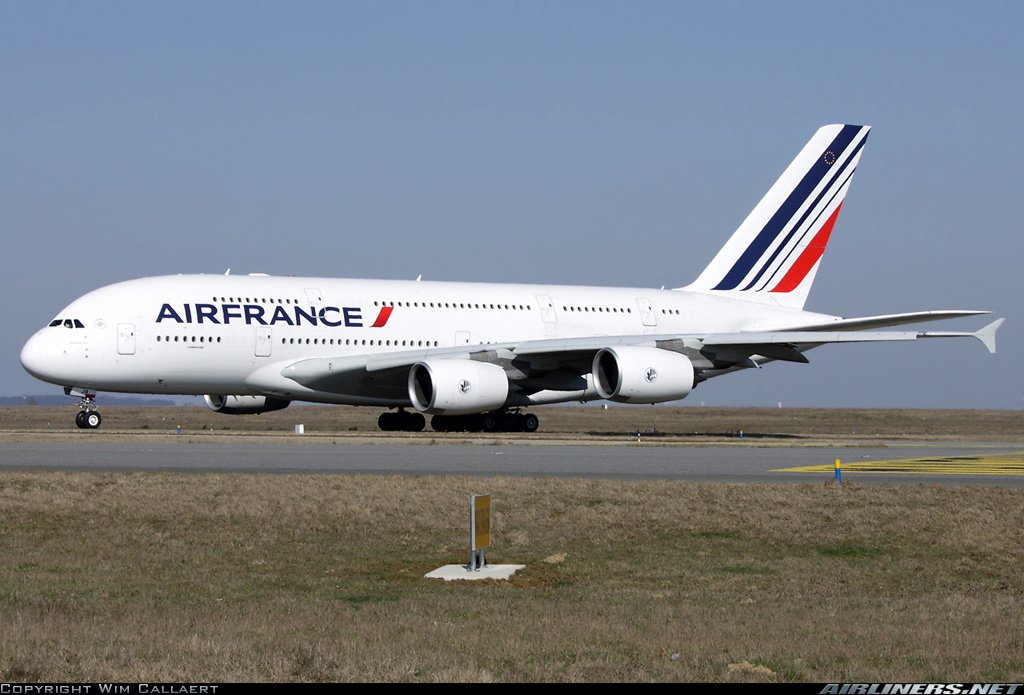
\includegraphics[width=0.3\linewidth]{figures/air/2.jpg}
    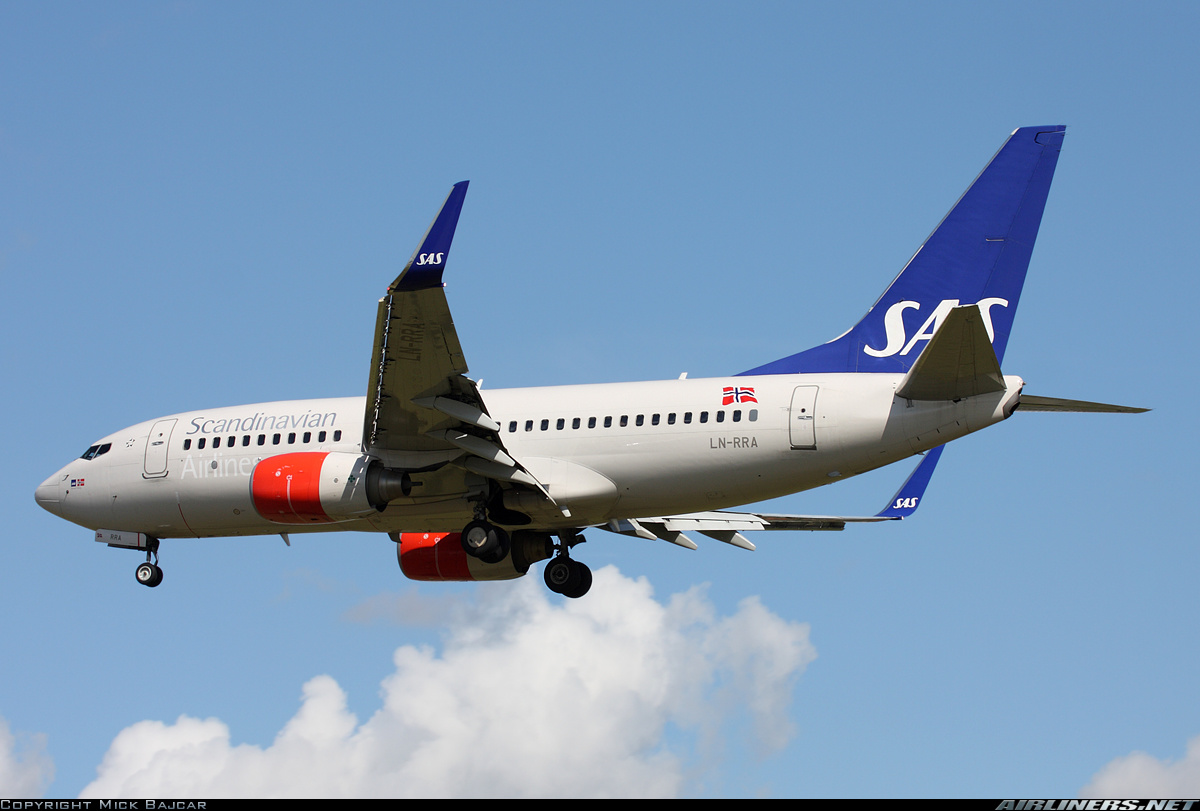
\includegraphics[width=0.3\linewidth]{figures/air/3.jpg}
  }
  \caption{数据集示例}
  \label{fig:datasets}
\end{figure}


\textbf{相比较的模型微调方法 } 为了展示随机标准化层在模型微调任务中的效果,我们选取了节~\ref{section:regularize}中的几种有代表性的模型微调方法进行比较:基线(Baseline)\textbf{$\bm{L_2}$范数},即不使用任何方法,直接利用预训练模型的参数作为初始化进行
微调训练;\textbf{$\bm{L_2}$-SP}\citep{xuhong2018explicit},通过将深度神经网络的网络参数,通过正则化的方式约束在预训练模型的网络参数附近,来缓解模型微调中容易遇到的灾难性遗忘;\textbf{DELTA}\citep{li2018delta},在特征图
维度通过一种有监督的注意力机制进行筛选,选出更适合进行模型微调的特征;\textbf{BSS}\citep{chen2019catastrophic},通过对深度神经网络生成表征的特征值进行正则化约束,来避免在模型微调中出现负迁移(Negative Transfer)。这三种方法均在发表
阶段取得了相应的模型微调任务上最好的效果,并且都能够有效地避免深度神经网络在微调阶段出现过拟合的现象。

\textbf{实验细节 } 模型微调部分的训练与验证遵循了相关工作\citep{xuhong2018explicit,li2018delta,chen2019catastrophic}中的设定,对于深度神经网络的特征提取器部分(Feature Extractor),使用预训练模型的参数作为其初始值,而对于与图像分类任务相关的最后一层
全连接层(Fully Connected Layer),则完全随机初始化从头开始训练。由于最后一层全连接层是随机初始化的,因此其学习率设为特征提取器部分的学习率的$10$倍。训练过程中本文采用随机梯度
下降(Stochasitc Gradient Descent,SGD)作为深度神经网络的优化器,动量值(Momentum)设置为$0.9$,并相应地加入了学习率衰减(Learning Rate Decay)策略。每组实验使用不同的随机种子
重复实验五次,结果取五次的平均值,并且汇报相应的标准差。对于训练数据与验证数据的划分,本文遵循了数据集原作者的划分方式,对于没有提供验证集的数据集,本文使用$20\%$的训练数据作为验证数据。
关于随机标准化层的超参数$p$,本文通过验证集上的效果进行选取。值得注意的是,在本节的绝大多数实验中选取$p=0.5$都能取得较好的效果,附录中详细提供了每个实验任务中$p$的选取值。


\subsection{实验结果}
\label{section:results}

三种细粒度分类数据集上的实验结果分别如表\ref{table:cub}、表\ref{table:car}、表\ref{table:air}所示。为了探索在数据量不足的情况下,随机标准化层对深度神经网络效果的影响,我们设计了
四种不同数据采样比例——$15\%$、$30\%$、$50\%$和$100\%$在训练集的数据上重新采样,分别对应着从小规模训练数据到中规模训练数据的范围。深度神经网络的结构统一采用ResNet-50\citep{he_deep_2016},使用由PyTorch官方提供的
预训练模型参数进行微调。

\begin{table*}[h]
	\begin{center}
	\caption{实验结果(CUB-200-2011)}
	\label{table:cub}
	\centering
      \begin{tabular}{lcccc}
          \toprule
          \multirow{2}*{方法} & \multicolumn{4}{c}{数据采样比例} \\
          & $15\%$ & $30\%$ & $50\%$ & $100\%$ \\
          \midrule
          Baseline($L_2$) & $45.25\pm0.12$ & $59.68\pm0.21$ & $70.12\pm0.29$ & $78.01\pm0.16$ \\
          $L_2$-SP \citep{xuhong2018explicit} & $45.08\pm0.19$ & $57.78\pm0.24$ & $69.47\pm0.29$ & $78.44\pm0.17$ \\
          DELTA \citep{li2018delta} & $46.83\pm0.21$ & $60.37\pm0.25$ & $71.38\pm0.20$ & $78.63\pm0.18$ \\
          BSS \citep{chen2019catastrophic} & $47.74\pm0.23$ & $62.03\pm0.29$ & $\textbf{72.56}\pm\textbf{0.17}$ & $78.85\pm0.31$  \\ 
          \cmidrule(r){1-5}
          \textbf{StochNorm} & $\textbf{50.14}\pm\textbf{0.19}$ & $\textbf{62.34}\pm\textbf{0.26}$ & $72.01\pm0.15$ &  $\textbf{79.58}\pm\textbf{0.13}$  \\
          \bottomrule
      \end{tabular}
	\end{center}
\end{table*}

\begin{table*}[h]
	\begin{center}
	\caption{实验结果(Standford Cars)}
	\label{table:car}
	\centering
      \begin{tabular}{lcccc}
          \toprule
          \multirow{2}*{方法} & \multicolumn{4}{c}{数据采样比例} \\
          & $15\%$ & $30\%$ & $50\%$ & $100\%$ \\
          \midrule
          Baseline($L_2$) & $36.77\pm0.12$ & $60.63\pm0.18$ & $75.10\pm0.21$ & $87.20\pm0.19$ \\
          $L_2$-SP \citep{xuhong2018explicit} & $36.10\pm0.30$ & $60.30\pm0.28$ & $75.48\pm0.22$ & $86.58\pm0.26$ \\
          DELTA \citep{li2018delta} & $39.37\pm0.34$ & $63.28\pm0.27$ & $76.53\pm0.24$ & $86.32\pm0.20$  \\
          BSS \citep{chen2019catastrophic} & $40.57\pm0.12$ & $64.13\pm0.18$ & $76.78\pm0.21$ & $\textbf{87.63}\pm\textbf{0.27}$  \\
          \cmidrule(r){1-5}
          \textbf{StochNorm} & $\textbf{41.08}\pm\textbf{0.17}$ & $\textbf{65.02}\pm\textbf{0.21}$ & $\textbf{77.39}\pm\textbf{0.26}$ & $87.35\pm0.22$  \\
          \bottomrule
      \end{tabular}
	\end{center}
\end{table*}

\begin{table*}[h]
	\begin{center}
	\caption{实验结果(FGVC Aircraft)}
	\label{table:air}
	\centering
      \begin{tabular}{lcccc}
          \toprule
          \multirow{2}*{方法} & \multicolumn{4}{c}{数据采样比例} \\
          & $15\%$ & $30\%$ & $50\%$ & $100\%$ \\
          \midrule
          Baseline($L_2$) & $39.57\pm0.20$ & $57.46\pm0.12$ & $67.93\pm0.28$ & $81.13\pm0.21$ \\
          $L_2$-SP \citep{xuhong2018explicit} & $39.27\pm0.24$ & $57.12\pm0.27$ & $67.46\pm0.26$ & $80.98\pm0.29$ \\
          DELTA \citep{li2018delta} & $42.16\pm0.21$ & $58.60\pm0.29$ & $68.51\pm0.25$ & $80.44\pm0.20$  \\
          BSS \citep{chen2019catastrophic} & $40.41\pm0.12$ & $59.23\pm0.31$ & $\textbf{69.19}\pm\textbf{0.13}$ & $81.48\pm0.18$  \\
          \cmidrule(r){1-5}
          \textbf{StochNorm} & $\textbf{42.63}\pm\textbf{0.18}$ & $\textbf{60.09}\pm\textbf{0.25}$ & $69.00\pm0.16$ & $\textbf{81.65}\pm\textbf{0.14}$  \\
          \bottomrule
      \end{tabular}
	\end{center}
\end{table*}

从表中的数据可以看出,StochNorm在目标域数据比较少的情况下($15\%$和$30\%$的数据采样比例)相较于最普通的模型微调方法$L_2$而言有非常明显的提升,同时在这两个极具挑战性的场景,$L_2$
非常容易遇到过拟合的问题。StochNorm在这两个场景下,相较于$L_2$有着平均$\textbf{4.10\%}$和$\textbf{3.23\%}$的提升,而相较于其他三种模型微调方法而言,StochNorm在绝大多数任务上都有提升。
本文提出的StochNorm主要通过引入正则化来缓解模型微调中过拟合的现象,因此在数据量较多的情况下($50\%$和$100\%$的数据采样比例)只能在一部分任务上有所提升,不过值得注意的是其余三种微调方法也都没能获得很明显的提升。

\subsection{分析实验}
\label{section:ablation}

\textbf{不同的深度神经网络结构 } 上一节的实验中,均采用了ResNet-50作为深度神经网络结构。但是在3.3节中提到,作为一种具有通用性的十分简洁的标准化层,随机标准化层也可以十分轻松地应用在其他不同的
深度神经网络结构中。本文在前一节提到的CUB-200-2011数据集上,在两种深度神经网络——VGG-16\citep{simonyan2015very}和Inception-V3\citep{szegedy2016rethinking}中加入随机标准化层进行了实验。VGG-16的特点是随着网络的加深,通道的数量不断
增大,而特征图的大小不断减少;Inception-V3的特点是将不同大小的卷积核并行使用,来实现多尺度的卷积操作。图\ref{fig:backbone}展示了在加入随机标准化层之后,深度神经网络在测试集上准确率
的绝对提升值。从图上可以看出,不同的神经网络中加入随机标准化层都能获得准确率上的提升,并且在数据量有限的情况下明显好于标准的模型微调,这也证明了随机标准化层能够轻松地与不同的使用了
标准化层的深度神经网络想结合,同时在模型微调阶段起到更好的正则化约束效果。

\begin{figure}
  \centering
  \subcaptionbox{使用不同的网络结构中\label{fig:backbone}}
    {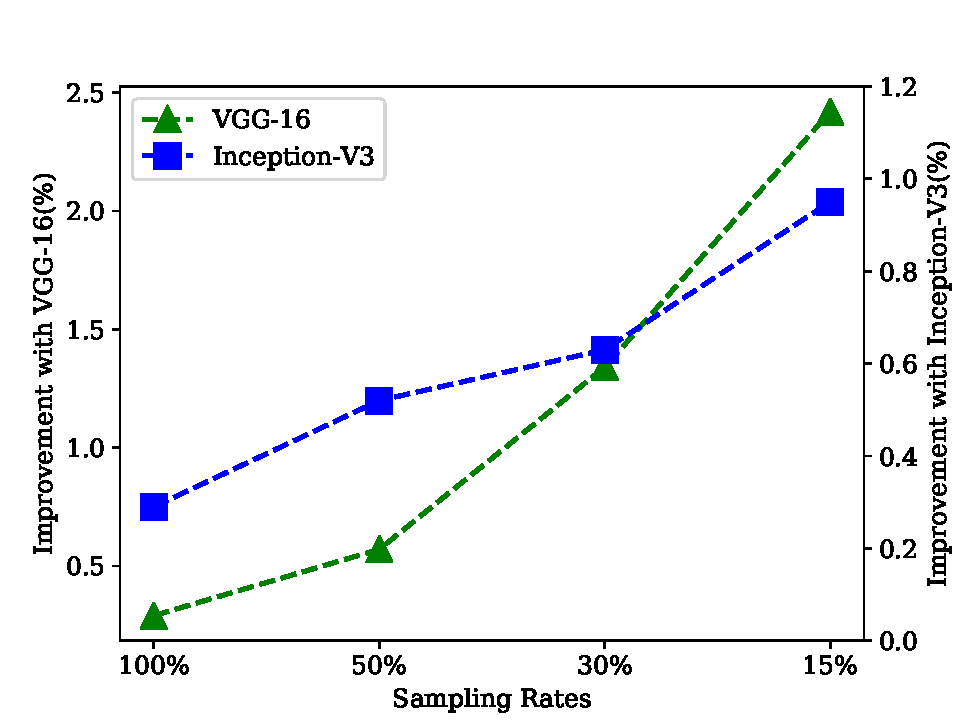
\includegraphics[width=0.48\linewidth]{figures/backbone.pdf}}
  \subcaptionbox{使用不同的初始化方法\label{fig:method}}
    {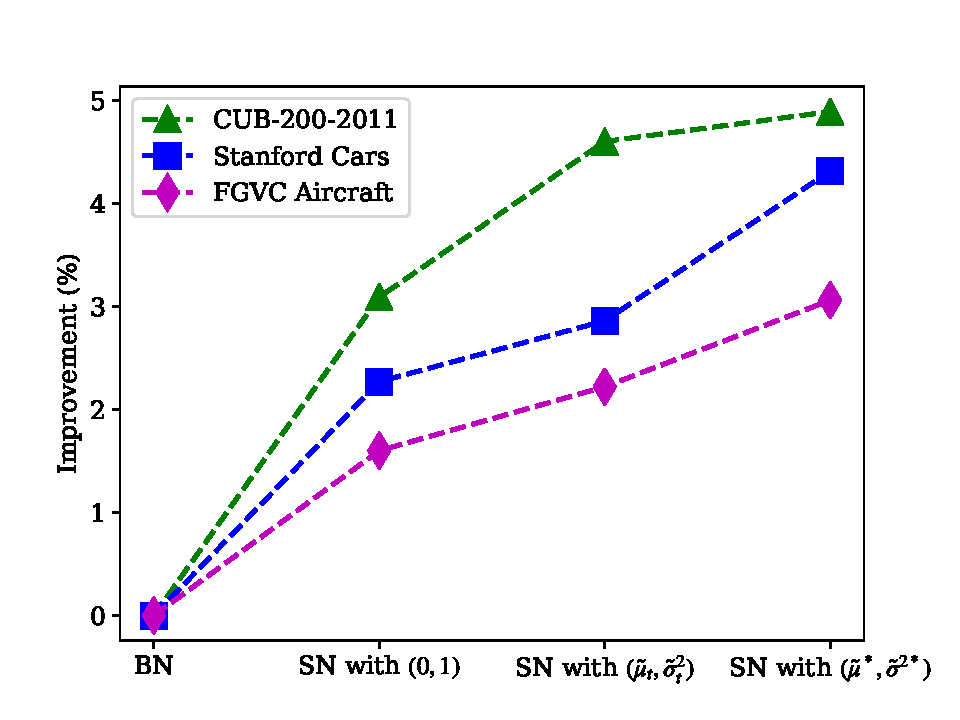
\includegraphics[width=0.48\linewidth]{figures/method.pdf}}
  \subcaptionbox{使用不同的分支选取概率\label{fig:p_acc}}
    {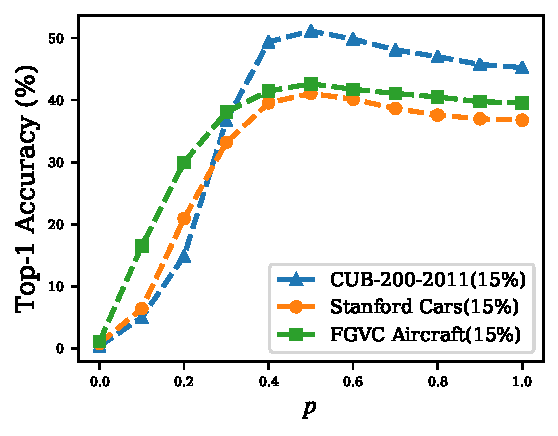
\includegraphics[width=0.48\linewidth]{figures/p_acc.pdf}}
  \caption{分析实验}
\end{figure}

\textbf{不同初始化方法的比较 } 为了更好的理解StochNorm,本文在~\ref{section:settings}中提到的三个细粒度分类数据集进行$15\%$采样,然后对StochNorm的几个变种进行了消融实验(Ablation Study)。StochNorm的主要创新点来自于双分支的设计以及在分支
间进行随机选择。这种设计也意味着,额外加入的使用$\tilde{\mu}, \tilde{\sigma}^2$进行标准化的分支,对网络的训练有很大的影响。由于在模型微调阶段,可以很自然地使用预训练模型中的$\tilde{\mu}^*, \tilde{\sigma}^{2^*}$作为其初始值,
本文在这里对不同的初始化方法进行了比较:
\begin{itemize}
  \item 使用$(\vec{0}, \vec{1})$作为初始值;
  \item 使用$\tilde{\mu}^*, \tilde{\sigma}^{2^*}$作为初始值;
  \item 使用$\tilde{\mu}_t, \tilde{\sigma}_t^2$作为初始值,其中$\tilde{\mu}_t, \tilde{\sigma}_t^2$使用目标域数据在预训练模型上前向反馈计算得到。
\end{itemize}

三个变种方法相对BatchNorm在三个数据集上的平均绝对提升如图~\ref{fig:method}所示。可以看出,$\tilde{\mu}^*, \tilde{\sigma}^{2^*}$的效果最好,而$(\vec{0}, \vec{1})$的效果最差。可以看出,尽管绝对提升没有随机选择的双分支结构高,但使用
包含着更多关于预训练数据以及模型指使的初始值,依然能够在模型微调阶段带来更多提升。

\textbf{不同的分支选取概率 } 作为StochNorm中唯一新增的超参数,分支选取概率$p$的选择对于模型最后的效果提升来说也十分关键,为了进一步分析超参数$p$对StochNorm效果的影响,我们在$15\%$采样的三个细粒度分类数据集上,
对$p$从$0.0$(即完全使用滑动平均估计的统计值进行标准化)到$1.0$(即BatchNorm)间隔$0.1$共$11$个取值分别进行了实验,实验结果如图~\ref{fig:p_acc}所示。可以看出,$p=0.5$在三个数据集上都取得了最好的效果,对于较大
的$p$而言,相对BatchNorm,即$p=0$而言,都有一定的提升,而较小的$p$则会导致网络不收敛,这与许多BatchNorm相关研究工作的结论一致。

% \begin{figure}
%   \centering
%   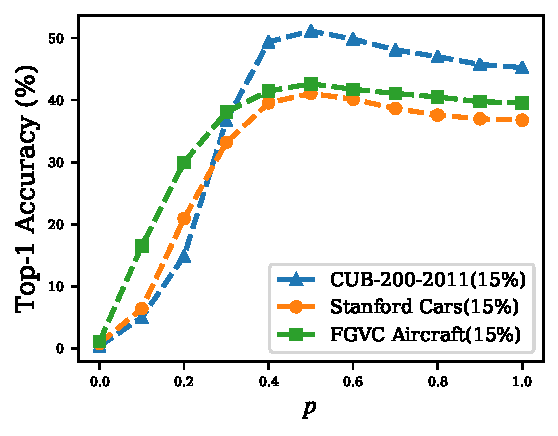
\includegraphics[width=0.5\linewidth]{figures/p_acc.pdf}
%   \caption{StochNorm中超参数$p$的选取对效果的影响}
%   \label{fig:p_acc}
% \end{figure}

\textbf{与模型微调方法相结合 } 本文在这一节的最后,将随机标准化层与前文提到的三种传统的模型微调方法进行结合,进一步展示了该方法的通用性。这里依旧选用节~\ref{section:settings}中三个细粒度分类数据集作为实验场景,预训练
模型依旧选择ResNet-50。实验结果如表\ref{table:combine_cub}、\ref{table:combine_cars}和\ref{table:combine_air}所示,可以很明显地看出,将随机标准化层与其他模型微调方法相结合,在大多数情况下能够进一步提升模型在测试集上的准确率。这是由于随机标准化层是一种网络结果层面
的方法,通过设计更合理地标准化层结构来实现对深度神经网络性能的提升。这与传统的在网络参数、网络特征层面进行正则化约束的模型微调方法是相互正交、相互弥补的。因此,两种方法相结合能够取得更好的效果也是理所当然。


\begin{table*}[htbp]
	\begin{center}
	\caption{与模型微调方法相结合的实验结果 (CUB-200-2011).}
	\label{table:combine_cub}
	\centering
        \begin{tabular}{lcccc} 
            \toprule
            \multirow{2}*{方法} & \multicolumn{4}{c}{数据采样比例} \\
            \cmidrule(lr){2-5}
             & $15\%$ & $30\%$ & $50\%$ & $100\%$ \\
            \midrule
            $L_2$-SP \citep{xuhong2018explicit} & $45.08\pm0.19$ & $57.78\pm0.24$ & $69.47\pm0.29$ & $78.44\pm0.17$ \\
            $L_2$-SP+\textbf{StochNorm} & $49.92\pm0.24$ & $60.48\pm0.12$ & $70.47\pm0.19$ & $79.24\pm0.11$  \\
            \cmidrule(r){1-5}
            DELTA \citep{li2018delta} & $46.83\pm0.21$ & $60.37\pm0.25$ & $71.38\pm0.20$ & $78.63\pm0.18$ \\
            DELTA+\textbf{StochNorm} & $49.27\pm0.31$ & $62.86\pm0.30$ & $72.78\pm0.16$ & $79.72\pm0.12$ \\
            \cmidrule(r){1-5}
            BSS \citep{chen2019catastrophic} & $47.74\pm0.23$ & $62.03\pm0.29$ & $72.56\pm0.17$ & $78.85\pm0.31$  \\ 
            BSS+\textbf{StochNorm} & $50.69\pm0.29$ & $64.10\pm0.18$ & $73.01\pm0.26$ & $79.91\pm0.14$  \\
            \bottomrule
        \end{tabular}
	\end{center}
\end{table*}

\begin{table*}[htbp]
	\begin{center}
	\caption{与模型微调方法相结合的实验结果 (Standford Cars).}
	\label{table:combine_cars}
	\centering
        \begin{tabular}{lcccc} 
            \toprule
            \multirow{2}*{方法} & \multicolumn{4}{c}{数据采样比例} \\
            \cmidrule(lr){2-5}
             & $15\%$ & $30\%$ & $50\%$ & $100\%$ \\
            \midrule
            $L_2$-SP \citep{xuhong2018explicit} & $36.10\pm0.30$ & $60.30\pm0.28$ & $75.48\pm0.22$ & $86.58\pm0.26$ \\
            $L_2$-SP+\textbf{StochNorm} & $40.50\pm0.23$ & $64.86\pm0.32$ & $77.34\pm0.11$ & $86.81\pm0.16$  \\
            \cmidrule(r){1-5}
            DELTA \citep{li2018delta} & $39.37\pm0.34$ & $63.28\pm0.27$ & $76.53\pm0.24$ & $86.32\pm0.20$  \\
            DELTA+\textbf{StochNorm} & $40.77\pm0.19$ & $65.67\pm0.17$ & $77.23\pm0.24$ & $86.51\pm0.15$ \\
            \cmidrule(r){1-5}
            BSS \citep{chen2019catastrophic} & $40.57\pm0.12$ & $64.13\pm0.18$ & $76.78\pm0.21$ & $87.63\pm0.27$  \\
            BSS+\textbf{StochNorm} & $44.04\pm0.21$ & $66.28\pm0.12$ & $78.03\pm0.18$ & $87.85\pm0.25$  \\
            \bottomrule
        \end{tabular}
	\end{center}
\end{table*}

\begin{table*}[htbp]
	\begin{center}
	\caption{与模型微调方法相结合的实验结果 (FGVC Aircraft).}
	\label{table:combine_air}
	\centering
        \begin{tabular}{lcccc} 
            \toprule
            \multirow{2}*{方法} & \multicolumn{4}{c}{数据采样比例} \\
            \cmidrule(lr){2-5}
             & $15\%$ & $30\%$ & $50\%$ & $100\%$ \\
            \midrule
            $L_2$-SP \citep{xuhong2018explicit} & $39.27\pm0.24$ & $57.12\pm0.27$ & $67.46\pm0.26$ & $80.98\pm0.29$ \\
            $L_2$-SP+\textbf{StochNorm} & $42.57\pm0.19$ & $60.16\pm0.28$ & $69.16\pm0.09$ & $81.12\pm0.16$  \\
            \cmidrule(r){1-5}
            DELTA \citep{li2018delta} & $42.16\pm0.21$ & $58.60\pm0.29$ & $68.51\pm0.25$ & $80.44\pm0.20$  \\
            DELTA+\textbf{StochNorm} & $44.10\pm.18$ & $60.13\pm0.22$ & $70.12\pm0.14$ & $81.03\pm0.15$ \\
            \cmidrule(r){1-5}
            BSS \citep{chen2019catastrophic} & $40.41\pm0.12$ & $59.23\pm0.31$ & $69.19\pm0.13$ & $81.48\pm0.18$  \\
            BSS+\textbf{StochNorm} & $43.89\pm0.30$ & $60.25\pm0.19$ & $69.41\pm0.26$ & $81.50\pm0.21$  \\
            \bottomrule
        \end{tabular}
	\end{center}
\end{table*}

\section{本章小结}

本章先介绍了广泛使用的BatchNorm的算法流程以及原理,之后介绍了一系列基于正则化约束的模型微调方法。之后本章在少量样本模型微调的场景下基于BatchNorm的不足与缺陷,设计了新的标准化层结构StochNorm,
并在三个细粒度分类数据集上进行了实验,证明了StochNorm的效果。接下来为了更全面地理解StochNorm,从不同的深度神经网络结构、不同的初始化方式、不同的超参数选取以及与不同的模型微调方法相结合四个角度
进行了分析性实验,进一步证明了StochNorm的有效性和通用性。